\section{Numerical implementations}
\subsection{Cutting the cell with $\alpha$ and $\phi$}
In this case, the normal direction $\mathbf{n}$ of certain cell is given by level set function $\phi$ and the void fraction $\alpha$ is given by volume of fluid function. This section means to explain the algorithm of finding such a plane with normal direction $\mathbf{n}$ that can cut the cell into the right void fraction $\alpha$. The locations of cell center point $\mathbf{x_i}$ and $N$ cell vertexes $\mathbf{x_{i_1}},...,\mathbf{x_{i_N}}$ are needed. Then we can get $N$ vectors $\mathbf{d_1},...,\mathbf{d_N}$ from cell center to $N$ cell vertexes. The projections of center point to vertex on the normal direction can be calculated as
\begin{equation}\label{21}
D_i=\mathbf{d_i}\cdot\mathbf{n},\quad for\quad i=1,...,N.
\end{equation}
Let us suppose the objective plane contain one of the vertexes and we can have a series of plane to cut the cell into different fractions (figure \ref{fig:multiplane}). Due to the cell's polyhedral characteristic, a piecewise function about the center cell distance and void fraction is drew in figure \ref{fig:piecewise}. The objective plane with the given void fraction $\alpha_i$ must have a certain distance $D^*$ to the center point $\mathbf{x_i}$ such that $\tilde{\alpha}(D^*)=\alpha_i $ .The first step is to find the point on the certain part of the piecewise function, which can be realized by comparing the void fraction value of vertexes and $\alpha^*$. Suppose the point $p$ is between point $k$ and $l$, such that ${D^*}\in[D_k,D_l]$. We use a cubic polynomial to fit this interval. The second step is to find the two trisection point in this interval, say, $m$ and $n$, and calculate the $\tilde{\alpha}(D_m)$ and $\tilde{\alpha}(D_n)$ in geometric way. Then we have four points for the four polynomial coefficients by solving a group of linear equations. Use LU decomposition to solve the linear $4\times4$ Vandermonde matrix system. Then use Newton's root finding method to find $D^*$ with the condition, $\left|\tilde{\alpha}(D^*)-\alpha_i\right|<\epsilon$. $\epsilon$ is a user-defined tolerance, typically set to $10^{-8}$.

\begin{figure}[htbp]
\centering
\subfigure[]{
\centering
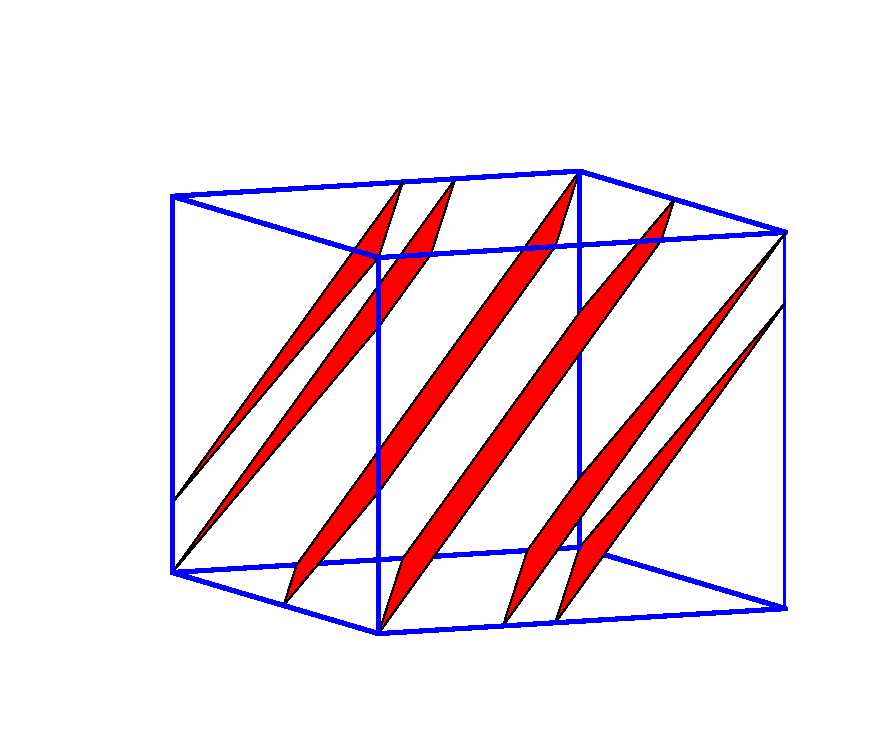
\includegraphics[width=0.4\textwidth]{multiplane.eps}
%\caption{fig1}
\label{fig:multiplane}
}
\quad
\subfigure[]{
\centering
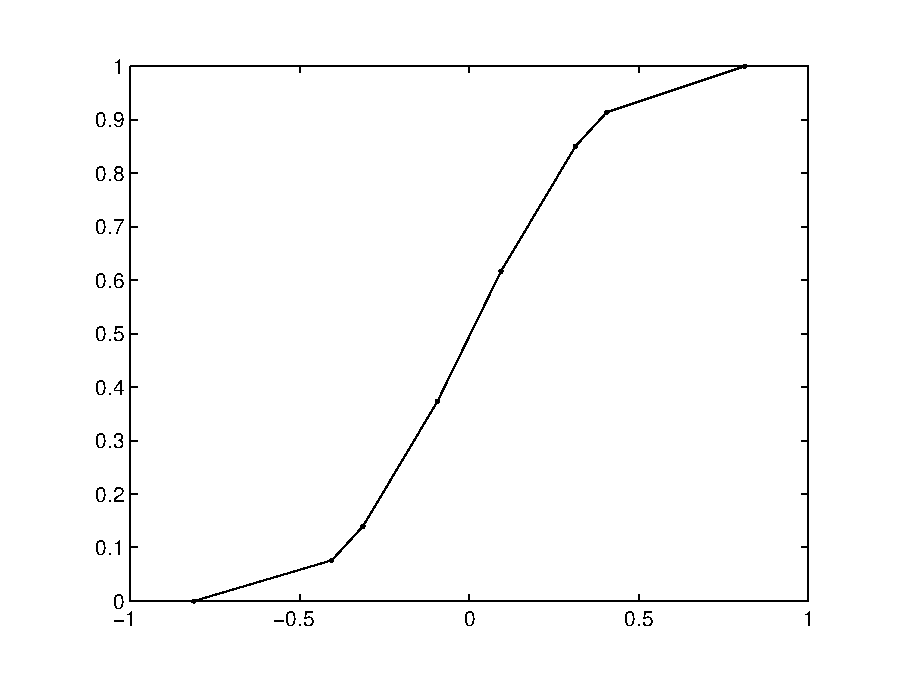
\includegraphics[width=0.4\textwidth]{piecewisefunction.eps}
\label{fig:piecewise}
%\caption{fig2}
}
%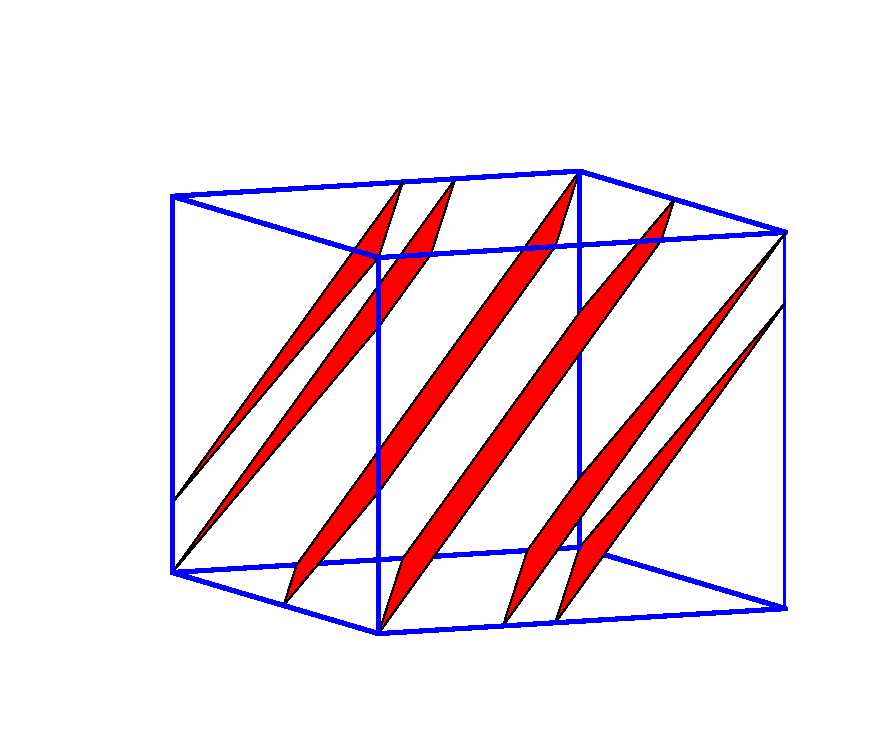
\includegraphics [width=0.5\textwidth]{multiplane.eps}
\caption{\subref{fig:multiplane} shows that planes pass different vertexes with the same normal direction. \subref{fig:piecewise} shows the cut volume and distance to the plane.}
\label{fig:multi}
\end{figure}

\subsection{Narrow band containing interface}
The cells that contain the interface are limited to where $H\in(\xi,1-\xi)$. $\xi$ is defined by users to confine the algorithm resolution, usually set as $0.0001$. The reason why uses Heaviside function rather than void fraction is that the interface defined by Heaviside function is more explicit and void fraction function more smeared. However, only interface cells are not enough to reconstruct the details of the interface. Level set method needs to build the signed distance function in the whole field, which can precisely capture the interface. Nonetheless, it takes too much computational resource and time to calculate on the whole field. So it is necessary to build a narrow band that has a thickness of two layers of grid like figure(\ref{fig:NarrowBand}). The first step is to sign all the interface cells with the flag "seed" and all the non-interface cell with the flag "away". The second step is to find the cells that share the vertexes of the "seed" cell. If the cells are signed with flags including "away" or "second layer", sign them with the flag "first layer". The third step is to traverse the cells that share the vertexes of the "first layer" cells. If the cells are signed with flags "away", sign them with the flag "second layer". Thus the narrow band that contains the interface and two-layers grids is built. The Heaviside function field and normal direction vector field can be limited in the narrow band to evade unnecessary computation.
\begin{figure}[htbp]
\centering
\includegraphics[width=0.5\textwidth]{band.eps}
\caption{The numbers in cells mean the flag. 0: "seed", 1:"first layer", 2:"second layer" and 4:"away"}
\label{fig:NarrowBand}
\end{figure}

\subsection{Reinitialization}
Reinitialization is actually the process of substitute $\tilde{\phi}(x,t)$ with another function $\phi(x,t)$ that has the same zero contour as $\tilde{\phi}(x,t)$ but the better property, $\left|\nabla\phi\right|=1$\cite{peng1999pde}. There are two ways to realize the process, including a direct, fast marching method(FMM)\cite{sethian1999level} and PDE-based method \cite{Sussman1994A} by converting it into a time-dependent Hamilton-Jacobi equation \ref{11}. As Sussman and Osher \textit{et al.} suggested in article \cite{Sussman1994A}, the sign function $sgn(x)$ can be approximated as the following equation,
\begin{equation}\label{22}
sgn(\tilde{\phi})=\frac{\tilde{\phi}}{\sqrt{{\tilde{\phi}}^2+\epsilon^2}},
\end{equation}
where $\epsilon$ means the thickness of the interface in this article. To solve the Hamilton-Jacobi equation (\ref{11}),with $sgn(\phi)$ approximated by (\ref{22}), there is a canonical monotone upwind scheme, Godunov's scheme, described in \cite{osher2006level,osher1991high} and the equation is discretized as the following,
\begin{equation}\label{23}
\phi^{n+1}_{i,j}=\phi^{n}_{i,j}-\Delta{\tau}sgn_\epsilon(\tilde{\phi})G(\phi^{n}_{i,j}),
\end{equation}
where $sgn_{\epsilon}(\tilde{\phi})$ is the approximation to equation(\ref{22}) and $G(\phi^{n}_{i})$ is defined as
\begin{equation}\label{24}
G(\phi^{n}_{i})=
\left\{
\begin{array}{ll}
\sqrt{max[(l^{+})^2,(r^{-})^2]+max[(s^{+})^2,(n^{-})^2]+max[(b^{+})^2,(t^{-})^2]}-1&{\tilde{\phi}_{i}>0} \\
\sqrt{max[(l^{-})^2,(r^{+})^2]+max[(s^{-})^2,(n^{+})^2]+max[(b^{-})^2,(t^{+})^2]}-1&{\tilde{\phi}_{i}<0}\\
0 & others 
\end{array}\right.
\end{equation}
The parameters in equation(24) show as follows,
\begin{equation}\label{25}
\begin{split}
&l=\sum_{j\in{\mathsf{F}}}{D_{i,j}}\max[\frac{\vec{x}_j-\vec{x}_i}{\left|{\vec{x}_j-\vec{x}_i}\right|}\cdot(-1,0,0),0]
\\
&r=-\sum_{j\in{\mathsf{F}}}{D_{i,j}}\max[\frac{\vec{x}_j-\vec{x}_i}{\left|{\vec{x}_j-\vec{x}_i}\right|}\cdot(1,0,0),0]
\\
&s=\sum_{j\in{\mathsf{F}}}{D_{i,j}}\max[\frac{\vec{x}_j-\vec{x}_i}{\left|{\vec{x}_j-\vec{x}_i}\right|}\cdot(0,-1,0),0]
\\
&n=-\sum_{j\in{\mathsf{F}}}{D_{i,j}}\max[\frac{\vec{x}_j-\vec{x}_i}{\left|{\vec{x}_j-\vec{x}_i}\right|}\cdot(0,1,0),0]
\\
&t=\sum_{j\in{\mathsf{F}}}{D_{i,j}}\max[\frac{\vec{x}_j-\vec{x}_i}{\left|{\vec{x}_j-\vec{x}_i}\right|}\cdot(0,0,-1),0]
\\
&b=-\sum_{j\in{\mathsf{F}}}{D_{i,j}}\max[\frac{\vec{x}_j-\vec{x}_i}{\left|{\vec{x}_j-\vec{x}_i}\right|}\cdot(0,0,1),0]
\\
&D_{i,j}=\frac{\phi_{i,j}-\phi_i}{\left|{\vec{x_j}-\vec{x}_i}\right|}, j\in{\mathsf{F}}
\\
&z^+=max[z,0], z^-=min[z,0],
\end{split}
\end{equation}
where $\mathsf{F}$ means the cells that share faces with cell $i$. The above algorithm uses the Godunov's scheme in unstructured grid, which is successfully applied in OpenFOAM$^{\textregistered}$. During the calculation, the number of the iteration steps are defined by users and controlled by two input parameters, "CFL" and "ENUM" in the "tranportProperties" dictionary. The max iteration number NITER is defined as $NITER=CFL\times{ENUM}$. Actually, the optimal step number is 10 and the level set function can reach a satisfied effect according to \cite{liu2017coupled}.

\subsection{Correction for mass conservation}
The continuous interface is firstly assumed at the iso-surface at $\alpha=0.5$. Then level set function is built to simulate the interface is at $\phi=0$. After the reinitialization process, the level set function needs to be corrected for the process slightly change the position of the interface to meet the mass conservative condition. The correction procedure takes advantage of cubic polynomial function to fit the relation of $\phi$ and total mass $M$. Dur to the narrow band, level set function $\phi$ is limited at $[min(\phi),max(\phi)]$. The first step of correction is to calculate the value of three points,$0.1max(\phi),0.05max(\phi),0.05min(\phi)$. Secondly, calculate the volume wrapped by the iso-value contours including the three points and zero points. Then there are four interpolation values for getting the cubic polynomial coefficients by solving a linear equation group. The detailed algorithms including LU decomposition and Newton's root finding method are the same as section 3.1 of how to getting the reconstructed interface position. After correction, the continuous, mass-conservative interface is obtained and ready for convection in the velocity field. 

\subsection{Numerical Discretization of level set equation}
In some articles like \cite{sun2010coupled,WANG201370}, the level set equation is not solved. And the level set function produced from the $\alpha$ field. However, it is testified in this article that not-solving the level set equation explicitly increase the distortion of the interface, because only the advection of void volume is not enough to calculate the normal direction at the next time step, let alone predict the position of the interface precisely. In this article, a third-order TVD-RK temporal scheme and semi-implicit third-order upwind WENO scheme or Vanleer scheme are used in solving the level set equation (\ref{10}).

\begin{equation}\label{26}
\begin{split}
&\phi^{(0)}=\phi_t\\
&\phi^{(1)}=\phi^{(0)}-\Delta{t}(\vec{u}\cdot\nabla)\phi^{(0)}\\
&\phi^{(2)}=\frac{3}{4}\phi^{(0)}+\frac{1}{4}\phi^{(1)}-\frac{1}{4}\Delta{t}(\vec{u}\cdot\nabla)\phi^{(1)}\\
&\phi_{t+\Delta{t}}=\frac{1}{3}\phi^{(0)}+\frac{2}{3}\phi^{(2)}-\frac{2}{3}\Delta{t}(\vec{u}\cdot\nabla)\phi^{(2)}
\end{split}
\end{equation}
The discretization of $(\vec{u}\cdot\nabla)\phi^{(0)}$ is easily to realize because the WENO scheme and Van Leer scheme are already coded in OpenFOAM$^{\textregistered}$, which are not the main work of this article and only need to add the source files and correctly write the dictionary, "fvScheme". 